\documentclass{article}

% Packages
\usepackage[utf8]{inputenc} % For modern characters
\usepackage{microtype} % For sexy kerning
\usepackage{mathtools} % For math stuff
\usepackage{amssymb} % For math symbols
\usepackage{tabularx} % For making tables
\usepackage{listings} % For writing code
\usepackage{fancyhdr} % Use a header
\usepackage{pdfpages} % Include PDFs

% Set the margins
\usepackage[scale=0.8, top=1in, bottom=1in]{geometry}

% Other front matter
\lstset{language=R} % Set listing language to R
\newcommand{\code}[1]{\texttt{#1}} % More readable for writing inline code.
\newcommand{\p}[1]{\paragraph{#1}} % Easier to type out for paragraph command
\newcommand{\tab}{\hspace*{3em}} % Set tab spaces
\pagestyle{fancy} % Makes Header Possible
{ %%% Header Set up
	\lhead{} % Set the left header to be blank
	\chead{} % Set the center header to be blank
	% Header for every page except the first two
	\rhead{Ben Foster | Homework 3 | April 24, 2015} % Name, assignment, date
}
\setcounter{tocdepth}{2} % Set Table of Contents Depth
\setlength{\parindent}{0pt} % Disable automatic indentation

%%%%%%%%%%%%%%%%%%%% Begin Document %%%%%%%%%%%%%%%%%%%%
\begin{document}

{ % Title page, table of contents, and page number setting
	\title{Probability and Statistics for Engineers Homework Three \\ TMATH 390}
	\author{Ben Foster\thanks{
		Institute of Technology, University of Washington Tacoma} \\
		Instructor: Julia Eaton}
	\date{April 24, 2015}
	\maketitle
	\thispagestyle{empty} % No page number at bottom
	\clearpage
	
	\pagenumbering{roman}
	\tableofcontents
	\clearpage
	\setcounter{page}{1}
	\pagenumbering{arabic}
}

%%%%%%%%%%%%%%%% Chapter Two Questions %%%%%%%%%%%%%%%%%%%

\section*{Problem 1} %%% DONE
\addcontentsline{toc}{section}{First Problem}

	From problem 2.45 on page 95 of the textbook: \\

	The accompanying normal quantile plot was constructed from a sample of 30 readings on 
	tension for mesh screens behind the surface of video display tubes used in computer monitors. 
	Does it appear plausible that the tension distribution is normal?
	
	\begin{figure}[!htb]
		\centering
		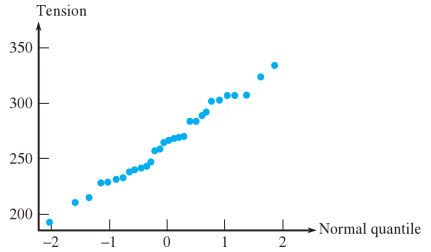
\includegraphics[width=4in]{img/Prob2_45Graph.jpg} 
		\caption{Problem 2.45 Graph}
		\label{fig:example}
	\end{figure}
	
	\p{Answer} In order for this to a Normal Distribution, the quantile plot shown above would have 
	to be a relatively straight line at around $45^\circ$. Since none of the points show too much 
	departure from linearity, then it appears fairly plausible that the distribution is Normal.
	
%%%%%%%%%%%%%%%% Chapter Three Questions %%%%%%%%%%%%%%%%%%

\clearpage
\section*{Problem 2} %%% DONE
\addcontentsline{toc}{section}{Second Problem}

	A study to assess the capability of subsurface flow wetland systems to remove biochemical 
	oxygen demand and various other chemical constituents resulted in the accompanying data on 
	$x =$ BOD mass loading (kg/ha/d) and $y =$ BOD mass removal (kg/ha/d) ("Subsurface Flow 
	Wetlands: A Performance Evaluation," Water Envir. Res., 1995: 244-247):
	
	\begin{table}[!htb]
	\begin{tabular}{ l c c c c c c c c c c c c c c }
		$x:$ & 3 & 8 & 10 & 11 & 13 & 16 & 27 & 30 & 35 & 37 & 38 & 44 & 103 & 142 \\
		$y:$ & 4 & 7 & 8 & 8 & 10 & 11 & 16 & 26 & 21 & 9 & 31 & 30 & 75 & 90 \\
	\end{tabular}
	\end{table}
	
	(a) Construct \code{boxplots} of both mass loading and mass removal, and comment on any 
	interesting features. \\ \\
	(b) Construct a scatter plot of the data and comment on any interesting features. \\ \\
	(c) Make the \code{qqplots} for $x$ and $y$, and comment on whether $x$ and/or $y$ could 
	have come from a Normal distribution.
	
	\p{Answer to a}
	In Figure 2 on the next page are the two Boxplots of $x$ and $y$ made in R. One interesting 
	feature is that there seem to be some correlating extremes and in general, the two boxplots 
	have pretty similar shapes and relative sizes, which may suggest some linearity of the quantile 
	plot.
	
	\p{Answer to b}
	In Figure 3 is the Scatterplot for $x$ vs. $y$. One interesting feature is that there are some 
	pretty extreme outliers and also that there is a tendency for $y$ to increase with $x$ meaning 
	that the correlation is positive.
	
	\p{Answer to c}
	In Figures 4 and 5 are the qqplots for both Mass Loading and Mass Removal. Both plots appear 
	to be slightly linear, but the extreme outliers are far off of where the line would be. I do not 
	believe that these data came from normal distributions.
	
	\clearpage
	\begin{figure}[htb]
	   \centering
	   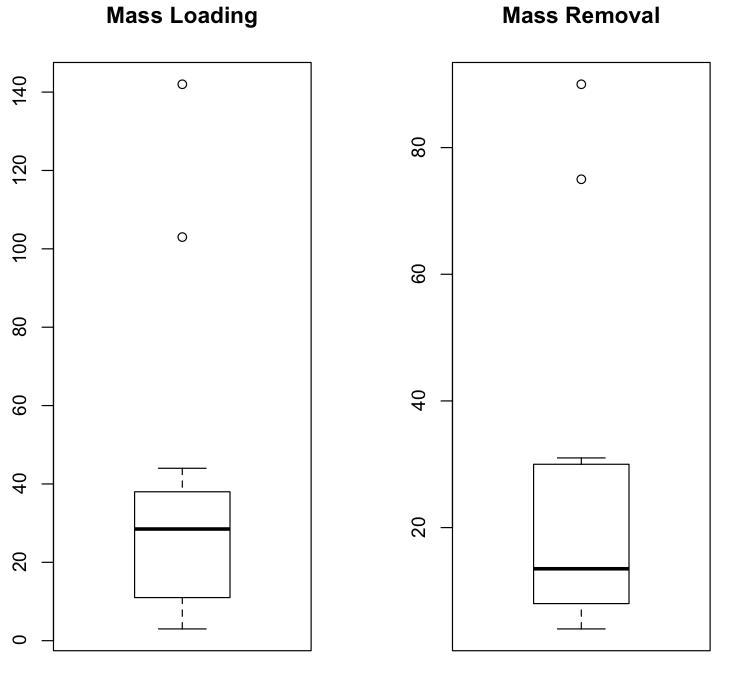
\includegraphics[width=\textwidth]{img/Problem2a.jpg} 
	   \caption{Boxplots of $x$ and $y$}
	   \label{fig:boxplots}
	\end{figure}
	
	\begin{figure}[htb]
	   \centering
	   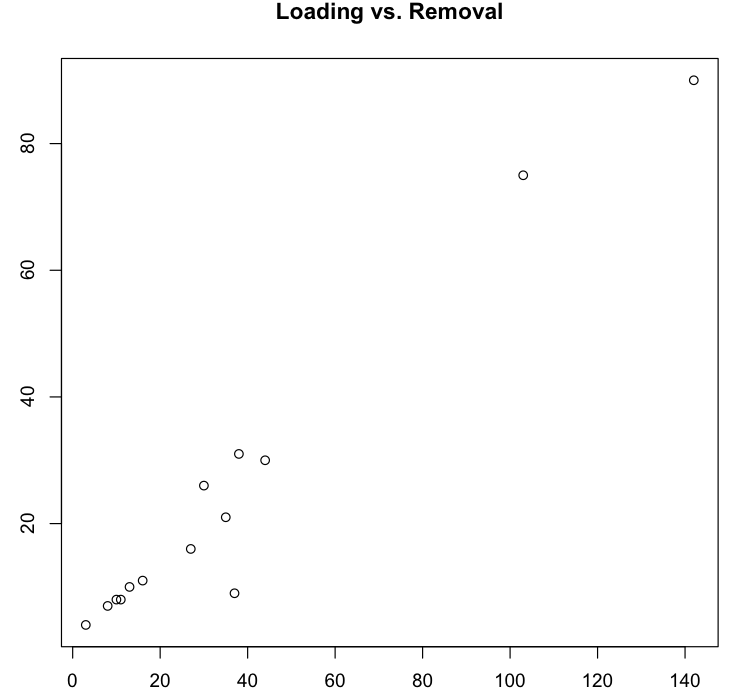
\includegraphics[width=\textwidth]{img/Problem2b.jpg} 
	   \caption{Scatterplot of $x$ vs. $y$}
	   \label{fig:scatterplot}
	\end{figure}
	
	\begin{figure}[htb]
	   \centering
	   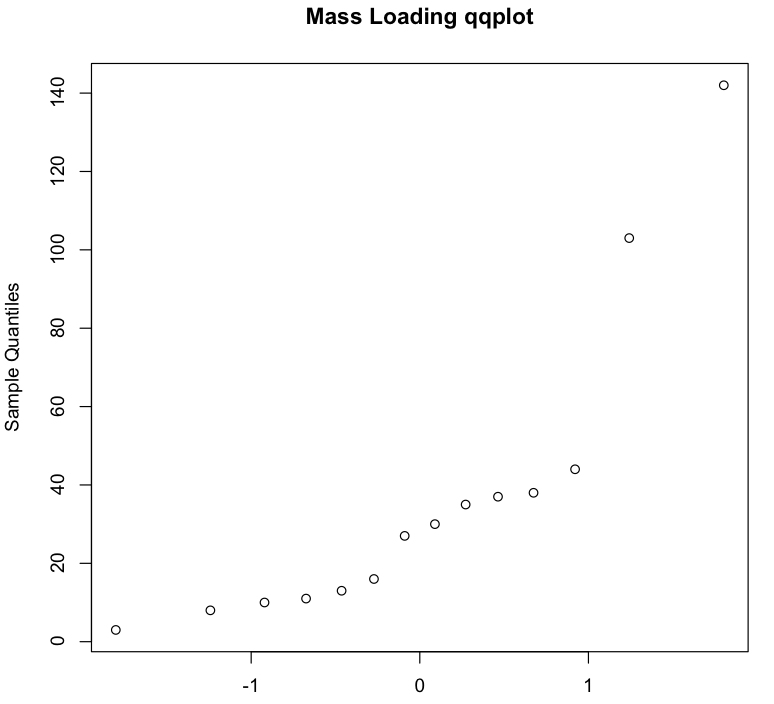
\includegraphics[width=\textwidth]{img/Problem2c_x.jpg} 
	   \caption{qqplot of Mass Loading}
	   \label{fig:loading_qqplot}
	\end{figure}
	
	\begin{figure}[htb]
	   \centering
	   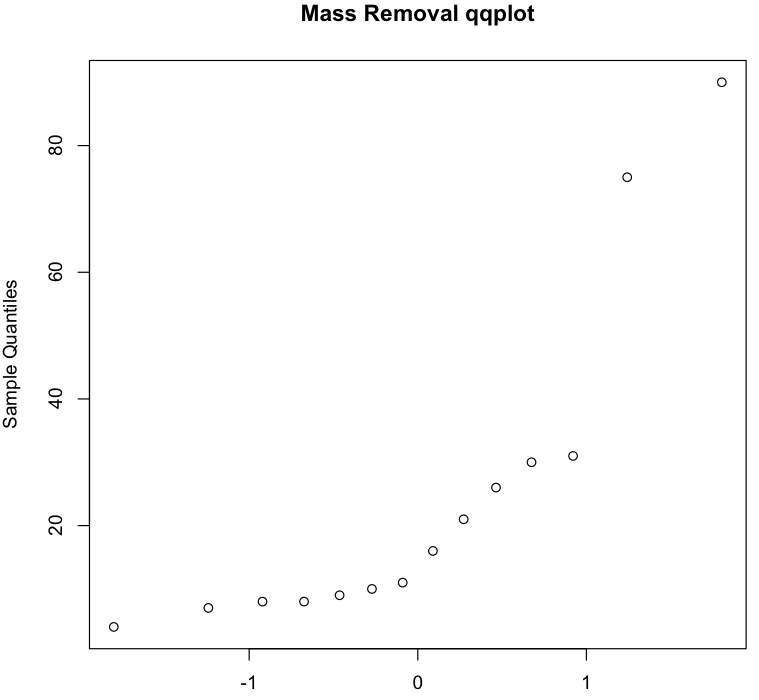
\includegraphics[width=\textwidth]{img/Problem2c_y.jpg} 
	   \caption{qqplot of Mass Removal}
	   \label{fig:removal_qqplot}
	\end{figure}

\clearpage
\section*{Problem 3} %%% DONE
\addcontentsline{toc}{section}{Third Problem}

	Here is the formula for Pearson's r:
	\[ r = \frac{1}{n-1}\sum_{i=1}^{n}\left(\frac{x_i - \bar{x}}{s_x}\right)\left(\frac{y_i - \bar{y}}{s_y}
	\right) \]
	
	(a) Start with the formula above, and show that it is equal to
	\[ r = \frac{\sum(x_i-\bar{x})(y_i-\bar{y})}{\sqrt{\sum(x_i-\bar{x})^2}\sqrt{\sum(y_i-\bar{y})^2}} \]
	
	(b) Start from part (a), and show that it is equal to
	\[ r = \frac{S_{xy}}{\sqrt{S_{xx}S_{yy}}} \]
	Where $S_{xx},S_{xy},S_{yy}$ are defined on page 110.
%	\[ S_{xx} = \sum x_i^2 - \frac{\left(\sum x_i\right)^2}{n} \]
%	\[ S_{yy} = \sum y_i^2 - \frac{\left(\sum y_i\right)^2}{n} \]
%	\[ S_{xy} = \sum x_iy_i - \frac{\left(\sum x_i\right)\left(\sum y_i\right)}{n} \]
	
	\p{Answer to a}
	\[ r = \frac{1}{n-1}\sum\left(\frac{x_i-\bar{x}}{s_x}\right)\left(\frac{y_i-\bar{y}}{s_y}\right) \]
	\[ = \frac{1}{n-1}\sum\left(\frac{(x_i-\bar{x})\sqrt{n-1}}{\sqrt{\sum(x_i-\bar{x})^2}}\right) 
	\left(\frac{(y_i-\bar{y})\sqrt{n-1}}{\sqrt{\sum(y_i-\bar{y})^2}}\right) \]
	\[ = \frac{n-1}{n-1}\sum\left(\frac{(x_i-\bar{x})}{\sqrt{\sum(x_i-\bar{x})^2}}\right) 
	\left(\frac{(y_i-\bar{y}}{\sqrt{\sum(y_i-\bar{y})}}\right) \]
	Since $\sqrt{\sum(x_i-\bar{x})^2}$ and $\sqrt{\sum(y_i-\bar{y})^2}$ are constants:
	\[ r = \frac{\sum(x_i-\bar{x})(y_i-\bar{y})}{\sqrt{\sum(x_i-\bar{x})^2}\sqrt{\sum(y_i-\bar{y})^2}} \]
	
	\p{Answer to b}
	Starting from the equation above:
	%%% Step 1
	\[ = \frac{\sum (x_iy_i - \bar{y}x_i - \bar{x}y_i + \bar{x}\bar{y})}
	{\sqrt{\sum(x_i^2 - 2\bar{x}x_i + \bar{x}^2)}\sqrt{\sum(y_i^2 - 2\bar{y}y_i + \bar{y}^2)}} \]
	%%% Step 2
	\[ = \frac{\sum x_iy_i - \bar{y}\sum x_i - \bar{x}\sum y_i + \bar{x}\bar{y}\sum 1}
	{\sqrt{\sum x_i^2 - 2\frac{\sum x_i}{n}\sum x_i + \sum\bar{x}^2}
	 \sqrt{\sum y_i^2 - 2\frac{\sum y_i}{n}\sum y_i + \sum\bar{y}^2}} \]
	%%% Step 3
	\[ = \frac{\sum x_iy_i - \frac{\sum y_i\sum x_i}{n} - \frac{\sum x_i\sum y_i}{n} + n\frac{\sum x_i
	\sum y_i}{n^2}}
	{\sqrt{\sum x_i^2 - 2\frac{\sum x_i}{n}\sum x_i + n\frac{(\sum x_i)^2}{n^2}}
	 \sqrt{\sum y_i^2 - 2\frac{\sum y_i}{n}\sum y_i + n\frac{(\sum y_i)^2}{n^2}}} \]
	%%% Step 4
	\[ = \frac{\sum x_iy_i - 2\frac{\sum y_i\sum x_i}{n} + \frac{\sum x_i\sum y_i}{n}}
	{\sqrt{\sum x_i^2 - 2\frac{\sum (x_i)^2}{n} + \frac{(\sum x_i)^2}{n}}
	 \sqrt{\sum y_i^2 - 2\frac{\sum (y_i)^2}{n} + \frac{(\sum y_i)^2}{n}}} \]
	%%% Step 5
	\[ = \frac{\sum x_iy_i - \frac{\sum x_i\sum y_i}{n}}
	{\sqrt{\sum x_i^2 - \frac{(\sum x_i)^2}{n}}
	 \sqrt{\sum y_i^2 - \frac{(\sum y_i)^2}{n}}} \]
	%%% Step 6
	\[ r = \frac{S_{xy}}{\sqrt{S_{xx}S_{yy}}} \] 

\section*{Problem 4} %%% DONE
\addcontentsline{toc}{section}{Fourth Problem}

	From problem 3.11 on page 116 of the textbook. \\

	Torsion during external rotation and extension of the hip may explain why acetabular labra tears 
	occur in professional athletes. The article "Hip Rotational Velocities During the Full Golf 
	Swing" (\textit{J. of Sports Sci. and Med.}, 2009: 296-299) reported on an investigation in which 
	lead hip internal peak rotational velocity ($x$) and trailing hip peak external rotational velocity 
	($y$) were determined for a sample of 15 golfers. Data provided by the article's authors was 
	used to calculate the following summary quantities:
	
	\[ \sum(x_i-\bar{x})^2 = 64,732.83 \]
	\[ \sum(y_i-\bar{y})^2 = 130,566.96 \]
	\[ \sum(x_i-\bar{x})(y_i-\bar{y}) = 44,185.87 \]
	
	Based on this, compute the sample correlation coefficient and interpret its value. How would 
	you characterize this correlation--as strong, moderate, or weak?
	
	\p{Answer} The sample correlation coefficient, or Pearson's r, is defined as:
	\[ r = \frac{\sum(x_i-\bar{x})(y_i-\bar{y})}{\sqrt{\sum(x_i-\bar{x})^2}\sqrt{\sum(y_i-\bar{y})^2}} \]
	Given the above values for $\sum(x_i-\bar{x})^2$, $\sum(y_i-\bar{y})^2$, and $\sum(x_i-\bar{x})
	(y_i-\bar{y})$, we get:
	\[ r = \frac{44,185.87}{\sqrt{64,732.83}\sqrt{130,566.96}} \]
	\[ r = 0.481 \]
	
	From this  value of r, I would characterize this correlation as moderately positive since $0 < r < 
	1$, but the value of r isn't very large.

\clearpage
\section*{Problem 5} %%% DONE
\addcontentsline{toc}{section}{Fifth Problem}

	From problem 3.16 on page 117 of the textbook. \\

	Suppose that $x$ and $y$ are positive variables and that a sample of $n$ pairs results in $r = 
	1$. If the sample correlation coefficient is computed for the $(x,y^2)$ pairs, will the resulting 
	value also be approximately 1? Explain.
	
	\p{Answer} 
	When looking at the scatterplot for a set of bivariate data with a Pearson Coefficient of 1, we 
	would see a perfectly straight line. If we plot the set of data $(x,y^2)$, then we would see a 
	curve, representing a slight parabolic shape. This will not produce a Pearson Coefficient of 1 
	but will be approximately 1 since the values are still close to being linear.

\section*{Problem 6} %%% DONE
\addcontentsline{toc}{section}{Sixth Problem}

	Compute the least squares line for data in Problem 2. Use the command \code{lm(y$\sim$x)} in 
	R.
	
	\p{Answer} By using the command in R, we get the value 0.6261 for our intercept and 0.6523 
	for our slope. \\
	
	In order to solve this by hand, we would use the equations given in the book:
	\[ b = \frac{S_{xy}}{S_{xx}} = \frac{\sum x_iy_i - \frac{(\sum x_i)(\sum y_i)}{n}}{\sum x_i^2 - 
	\frac{(\sum x_i)^2}{n}} \]
	\[ a = \bar{y} - b\bar{x} \]
	Where
	\[ b = \frac{ 25825 - \frac{(517)(346)}{14}}{39095 - \frac{(517)^2}{14}} \]
	\[ b = 0.6522902004 \]
	\[ a = 24.714 - (0.6523)(36.928) \]
	\[ a = 0.626140458 \]
	Therefore the equation of the least squares line is:
	\[ \hat{y} = 0.6261 + 0.6523 x \]
	
\clearpage
\section*{Problem 7} %%% DONE
\addcontentsline{toc}{section}{Seventh Problem}

	From problem 3.25 on page 131 of the textbook. \\
	
	Two important properties of a soil are its initial void ratio ($e_0$, a measure of soil porosity) and 
	its compression index ($C_c$, an indicator of soil compressibility). The article "Consolidation 
	and Hydraulic Conductivity of Zeolite-Amended Soil-Bentonite Backfills" (\textit{J. Geotech. 
	Geoenviron. Engr.}, 2012: 15-25) reported the following data (read from a graph) for the $C_c$ 
	and $e_0$ variables for sand-bentonite backfills with varying amounts and types of zeolites:
	
	\begin{table}[!htb]
	\begin{tabular}{ l c c c c c c }
		$e_0:$ & 0.988 & 1.018 & 1.058 & 1.070 & 1.085 & 1.145 \\
		$C_c:$ & 0.19 & 0.20 & 0.20 & 0.22 & 0.23 & 0.24 \\
	\end{tabular}
	\end{table}
	
	(a) Using $C_c$ as the response and $e_0$ as the explanatory variable, create the 
	corresponding scatterplot. Do the values of $C_c$ appear to be perfectly linearly related to the 
	$e_0$ values? Explain. \\ \\
	(b) Determine the equation of the least squares line. \\ \\
	(c) What proportion of the observed variation in the compression index can be attributed to the 
	approximate linear relationship between the two variables? \\ \\
	(d) Predict the value of the compression index when the initial void ratio is 1.10. Would you 
	feel comfortable using the least squares line to predict the compression index when the initial 
	void ratio is 0.80? Explain.
	
	\p{Answer to a}
	\begin{figure}[!htb]
	   \centering
	   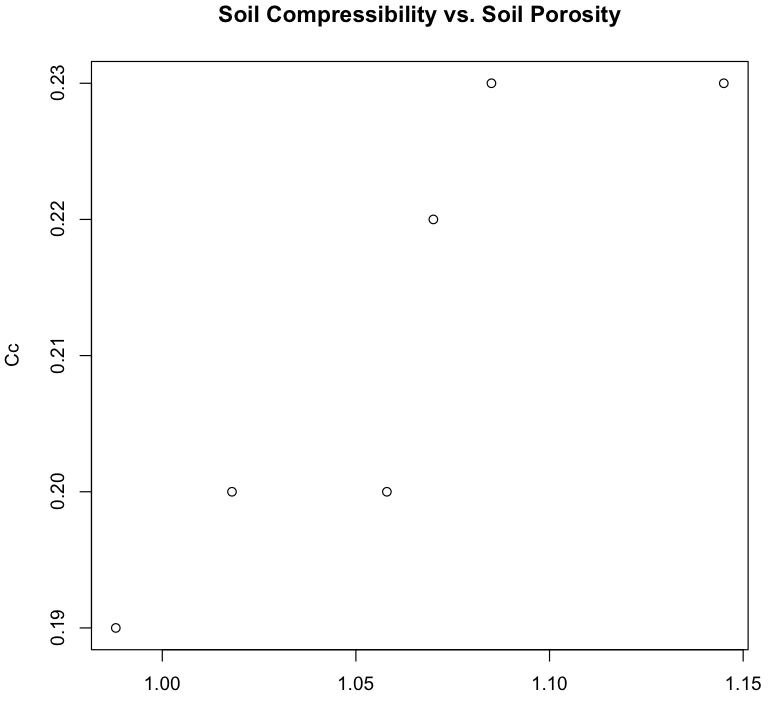
\includegraphics[width=4in]{img/Prob7a.jpg} 
	   \caption{$C_c$ vs. $e_0$}
	   \label{fig:example}
	\end{figure}
	From observing the scatterplot, we can see that the values of $C_c$ and $e_0$ are not 
	perfectly linearly related. If they were perfectly linearly related, then we would see the points 
	form a more straight line.
	
	\p{Answer to b}
	Using the equation $\hat{y} = a + bx$, we need to find the intercept $a$ and the slope $b$:
	\[ b = \frac{S_{xy}}{S_{xx}} = \frac{\sum x_iy_i - \frac{(\sum x_i)(\sum y_i)}{n}}{\sum x_i^2 - 
	\frac{(\sum x_i)^2}{n}} \]
	\[ b = \frac{1.36267 - \frac{(6.364)(1.28)}{6}}{6.765 - \frac{(6.364)^2}{6}} \]
	\[ b = 0.3367 \]
	\[ a = \frac{\sum y_i}{n} - b\frac{\sum x_i}{n} \]
	\[ a = 0.2133 - (0.3367)(1.061) \]
	\[ a = -0.1438 \]
	The equation of the least squares line is:
	\[ \hat{y} = -0.1438 + 0.3367x \]
	
	\p{Answer to c}
	The \textbf{Coefficient of Determination} is the proportion of variation in the observed y values 
	that can be attributed to (or explained by) a linear relationship between $x$ and $y$. The 
	coefficient of determination is described by:
	\[ r^2 = 1 - \frac{\text{SSResid}}{\text{SSTo}} \]
	\[ \text{SSResid} = \sum(y_i-\hat{y}_i)^2 = \text{SSTo} - bS_{xy} \]
	\[ \text{SSTo} = S_{yy} \]
	\[ b = \frac{\sum x_iy_i - \frac{(\sum x_i)(\sum y_i)}{n}}{\sum x_i^2 - \frac{(\sum x_i)^2}{n}} \]
	\[ b = \frac{1.36267 - 1.357653}{6.764982 - 6.750083} \]
	\[ b = 0.336734 \]
	\[ \text{SSTo} = \sum y_i^2 - \frac{(\sum y_i)^2}{n} \]
	\[ \text{SSTo} = 0.275 - 0.2730667 = 0.0019333 \]
	\[ S_{xy} = \sum x_iy_i - \frac{(\sum x_i)(\sum y_i)}{n} \]
	\[ S_{xy} = 1.36267 - 1.357653 \]
	\[ S_{xy} = 0.005017 \]
	\[ \text{SSResid} = 0.0019333 - (0.336734)(0.005017) \]
	\[ \text{SSResid} = 0.0002439055 \]
	\[ r^2 = 1 - \frac{0.0002439055}{0.0019333} \]
	\[ r^2 = 0.8738398 \]
	
	\p{Answer to d}
	To find the value of the compression index when the initial void ratio is 1.10, we have to use the 
	equation from part b:
	\[ \hat{y} = -0.1438 + 0.3367x \]
	And substitute 1.10 in for $x$:
	\[ \hat{y} = -0.1438 + 0.3367(1.10) \]
	In this case:
	\[ \hat{y} = 0.22657 \]
	So the value of the compression index when the initial void ratio is 1.10 is approximately 
	0.2266. I would not feel comfortable using the least squares line to predict the compression 
	index when the initial void ratio is 0.80 because it is below the lowest initial void ratio value and 
	once we start estimating values below or above the data set, then the chances of getting false 
	data can be pretty high.
	
\clearpage
\section*{Problem 8} %%% DONE
\addcontentsline{toc}{section}{Eighth Problem}

	Let
	\[ MSE = \frac{1}{n}\sum_{i=1}^{n}(y_i-\alpha-\beta x_i)^2 \]
	Set $\frac{\partial}{\partial\alpha}MSE = 0$, and derive the equation
	\[ \bar{y} - \alpha - \beta\bar{x} = 0 \]
	
	\p{Answer} Note: throughout this problem, $\sum_{i=1}^{n} = \sum$ for ease of writing.
	\[ \frac{\partial}{\partial\alpha}MSE = \frac{1}{n} \sum (y_i - \alpha - \beta x_i)^2 \]
	Using the chain rule:
	\[ 0 = \frac{1}{n}\sum 2(y_i-\alpha-\beta x_i)(-1) \]
	\[ 0 = \frac{1}{n}\sum (y_i - \alpha - \beta x_i) \]
	\[ 0 = \sum\frac{y_i}{n} - \sum\frac{\alpha}{n} - \sum\frac{\beta x_i}{n} \]
	\[ 0 = \bar{y} - \alpha - \beta\bar{x} \]


\section*{Problem 9} %%% Finish reading chapter
\addcontentsline{toc}{section}{Ninth Problem}

	In homework 1, you collected data which included data on 2 continuous variables. Call them $x
	$ and $y$, depending on which variable you want to predict from the other. That data is below:
	
	\begin{table}[!htb]
	\centering
	\begin{tabular}{ | c || c | c | c | c | } \hline
		Artist & Genre & Gender & Avg. length of song & Avg. $\frac{words}{song}$ \\ \hline \hline
		Jimi Hendrix & Classic Rock & Male & 7.35 min & 189.4 \\ \hline % 1
		Madonna & Pop & Female & 5.22 min & 120.2 \\ \hline % 2
		Skrillex & Dubstep & Male & 4.45 min & 13.7 \\ \hline % 3
		Eminem & Rap & Male & 6.14 min & 428.38 \\ \hline % 4
		Aesop Rock & Rap & Male & 7.78 min & 932.2 \\ \hline % 5
		Sia & Pop/Rock & Female & 4.69 min & 279.9 \\ \hline % 6
		Lorde & Pop & Female & 3.58 min & 155.01 \\ \hline % 7 
		Beck & Alt Rock & Male & 4.57 min & 180.34 \\ \hline % 8
		R. Kelly & R\&B & Male & 4.38 min & 210.23 \\ \hline % 9
		James Brown & R\&B & Male & 5.27 min & 280.56 \\ \hline % 10
	\end{tabular}
	\caption{Solo Artists}
	\label{tab:solo_artists}
	\end{table}
	
	We will have the average length of the song be our $x$ value and the average $\frac{words}
	{song}$ will be our $y$ value.
	
	(a) Produce the scatterplot of $x$ vs. $y$, and interpret. \\ \\
	(b) Compute the correlation coefficient between $x$ and $y$, and interpret. \\ \\
	(c) Perform linear regression to estimate the regression coefficients, and interpret them. \\ \\
	(d) Draw the regression line on the scatterplot of part (a). Does it look right? \\ \\
	(e) Compute $R^2$ and interpret.
	
	\clearpage
	\p{Answer to a}
	\begin{figure}[!htbp]
	   \centering
	   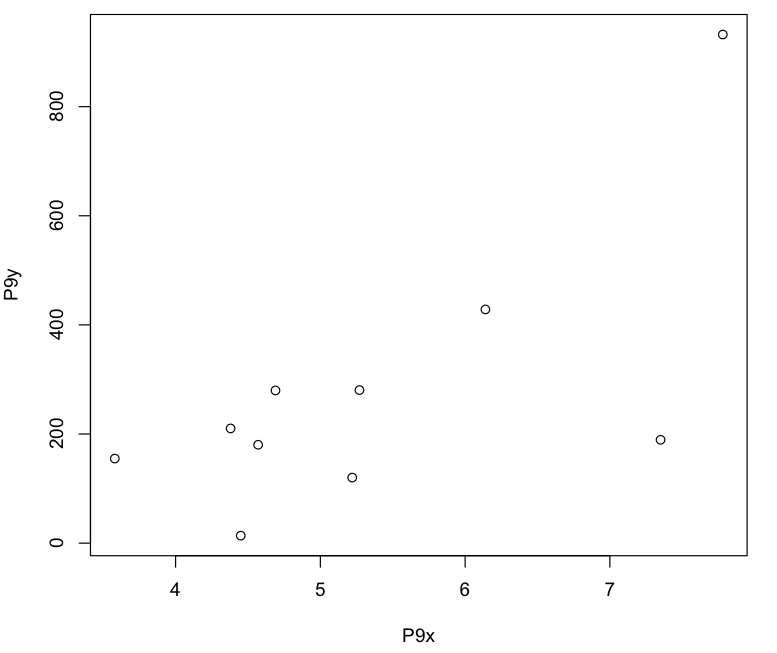
\includegraphics[width=\textwidth]{img/Prob9a.jpg} 
	   \caption{$\frac{Words}{Minute}$ vs. Song Length}
	   \label{fig:problem9_a}
	\end{figure}
	
	The scatterplot produced (shown in Figure 7) shows that there is a pretty strongly positive 
	correlation between $x$ and $y$.
	
	\clearpage
	\p{Answer to b}
	Given the correlations coefficient:
	% \bar{x} = 5.343, \bar{y} = 278.992
	\[ r = \frac{\sum(x_i-\bar{x})(y_i-\bar{y})}{\sqrt{\sum(x_i-\bar{x})^2}\sqrt{\sum(y_i-\bar{y})^2}} \]
	\[ \sum(x_i-\bar{x})^2 = 16.47961 \]
	\[ \sum(y_i-\bar{y})^2 = 582454.2 \]
	\[ \sum(x_i-\bar{x})(y_i-\bar{y}) = 2147.905 \]
	
	\[ r = \frac{2147.905}{\sqrt{16.47961}\sqrt{582454.2}} \]
	\[ r = 0.6933 \]
	
	Since the value of r is in the upper ranges, then we can now safely say that there is a strongly 
	positive correlation between our $x$ and $y$ values.
	
	\p{Answer to c} %%% This might be wrong
	To find the regression coefficients, we can use R and type in the command \code{lm($y\sim x
	$)}. 
	Doing this, we end up with:
	
	\begin{figure}[!htb]
		\centering
		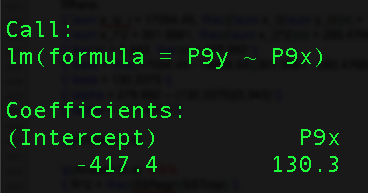
\includegraphics[width=2in]{img/Prob9c.jpg}
		\caption{Screenshot of regression coefficients}
		\label{fig:Problem9_c}
	\end{figure}
	
	By hand we would use the equations below and solve for $\alpha$ and $\beta$:
	\[ \beta = \frac{S_{xy}}{S_{xx}} = \frac{\sum x_iy_i - \frac{(\sum x_i)(\sum y_i)}{n}}{\sum x_i^2 - 
	\frac{(\sum x_i)^2}{n}} \]
	\[ \alpha = \bar{y} - \beta\bar{x} \]
	Where:
	\[ \sum x_iy_i = 17054.45, \frac{(\sum x_i)(\sum y_i)}{n} = 14906.54 \]
	\[ \sum x_i^2 = 301.9561, \frac{(\sum x_i)^2}{n} = 285.4765\]
	\[ \bar{x} = 5.343, \bar{y} = 278.992 \]
	\[ \beta = \frac{17054.45 - 14906.54}{301.9561 - 285.4765} \]
	\[ \beta = 130.3375 \]
	\[ \alpha = 278.992 -- (130.3375)(5.343) \]
	\[ \alpha = -417.4013 \]
	
	\clearpage
	\p{Answer to d} The line of regression looks correct.
	\begin{figure}[!htb]
	   \centering
	   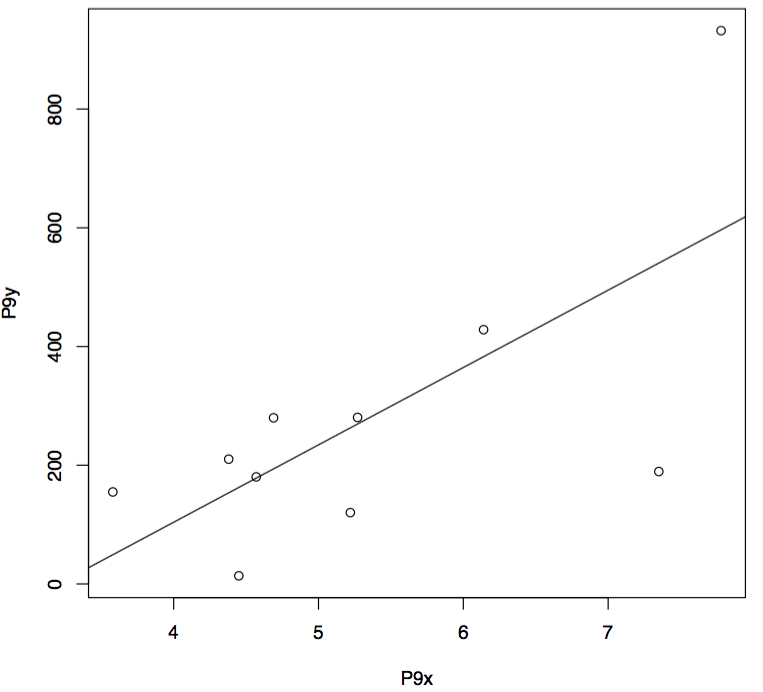
\includegraphics[width=\textwidth]{img/Prob9d.jpg} 
	   \caption{Regression Line of the Scatterplot}
	   \label{fig:problem9_d}
	\end{figure}
	
	\p{Answer to e} %%%
	%\[ R^2 = \frac{SSRegr}{SSTotal} \]
	%Proportion of variation in y explained by regression.
	%SSTotal = SSE + SSRegression
	Using $r$ from part b, we can see that $r^2 = 0.4806416$. Since the value is around 50\% we 
	can say that about half of the variation observed in $y$ is attributable to the linear relationship 
	between $x$ and $y$.

\end{document}